%%%%%%%%%%%%%%%%%%%%%%%%%%%%%%%%%%%%%%%%%
% DOCUMENTACION PASANTIA EN SONDA URUGUAY
% ING. JUAN BRAGA
% MAESTRÍA EN INGENIERÍA ELÉCTRICA, UDELAR
% JUNIO 2016
%%%%%%%%%%%%%%%%%%%%%%%%%%%%%%%%%%%%%%%%%

%----------------------------------------------------------------------------------------
%	PACKAGES AND DOCUMENT CONFIGURATIONS
%----------------------------------------------------------------------------------------

\documentclass{article}

\usepackage[version=3]{mhchem} % Package for chemical equation typesetting
\usepackage{siunitx} % Provides the \SI{}{} and \si{} command for typesetting SI units
\usepackage[spanish]{babel}
\selectlanguage{spanish}
\usepackage[utf8]{inputenc}
\usepackage{graphicx} % Required for the inclusion of images
\usepackage{natbib} % Required to change bibliography style to APA
\usepackage{amsmath} % Required for some math elements 

\setlength\parindent{0pt} % Removes all indentation from paragraphs

\renewcommand{\labelenumi}{\alph{enumi}.} % Make numbering in the enumerate environment by letter rather than number (e.g. section 6)

%\usepackage{times} % Uncomment to use the Times New Roman font

%----------------------------------------------------------------------------------------
%	DOCUMENT INFORMATION
%----------------------------------------------------------------------------------------

\title{\textbf{Desarrollo de módulo de procesamiento de audio en tiempo real con aplicación a seguridad urbana}\\ \textsc{Pasantía Laboral en SONDA Uruguay}\\
\large \textsc{Maestría en Ingeniería Eléctrica} del \textit{Instituto de Ingeniería Eléctrica, Facultad de Ingeniería, Universidad de la República, Uruguay.}}

\author{\textit{Ing. Juan Braga}}
\date{\today}

\begin{document}

\maketitle 

\begin{center}
\begin{tabular}{l r}
\medskip
\textsc{Período:} & \textsc{Diciembre 2015 a Marzo 2016}\\ % Date the experiment was performed
\textsc{Docente Responsable:} & \textit{Msc. Ing. Guillermo Carbajal} \\ 
\textsc{Responsable SONDA Uruguay:} & \textit{Nestor Rossi}, Gerente de Proyectos  \\
\textsc{Equipo de SONDA Uruguay:} & \textit{Ing. Florencia Lanzaro} \\ & \textit{Msc. Ing. Guillermo Carbajal} \\ 
\end{tabular}
\end{center}

%----------------------------------------------------------------------------------------
%	ABSTRACT
%----------------------------------------------------------------------------------------

\begin{abstract}
El presente informe tiene como objetivo la documentación del desarrollo realizado en SONDA Uruguay en el período de Diciembre 2015 a Marzo 2016, para su aprobación en créditos de la Maestría en Ingeniería Eléctrica de la UdelaR. Se detalla sobre un módulo de procesamiento de audio en tiempo real, para funcionamiento embebido en un software de analíticas para seguridad urbana, desarrollado en su totalidad por el equipo de Ingenieros de SONDA Uruguay. 
\end{abstract}

%----------------------------------------------------------------------------------------
%	SECTION 1
%----------------------------------------------------------------------------------------

\section{Introducción}
El monitoreo en tiempo real de las actividades humanas para Seguridad Urbana se ha vuelto masivo con el pasar de los últimos años a nivel mundial. La cantidad de sensores distribuidos por las ciudadades ha crecido enormemente. Es en los centros de monitoreo, donde confluyen los sensores colocados por la ciudad, que surge la necesidad de automatizar los procesos de visualización y control para hacer la operativa más eficiente \citep{Crocco:2016:ASS:2891449.2871183}. En este escenario es donde SONDA Uruguay motiva el desarrollo de un software de analíticas de audio y video, para el monitoreo automático en tiempo real de los espacios urbanos.   

\subsection{Sobre SONDA Uruguay}
SONDA Uruguay S.A. es fundamentalmente una empresa de servicios y proyectos de integracion de sistemas y provision de plataformas en el campo de las tecnologías de la información. Actualmente SONDA Uruguay S.A. está trabajando en proyectos de I+D en el area de tratamiento de señales, particularmente audio y video. 

\subsection{Sobre el equipo de trabajo}
El equipo de desarrollo en su totalidad esta conformado por 8 personas, profesionales y estudiantes de Ingeniería en Sistemas y Eléctrica, que complementan la rama de computación científica con las buenas prácticas de programación y manejo de arquitectura de software para aplicaciones críticas de gran volúmen de datos.  

\subsection{Sobre el software de analíticas de audio y video}
El software de analíticas actualmente forma parte de la tecnología implantada en el Centro de Monitoreo (CM) del Ministerio del Interior, en el proyecto Ciudad Segura.  Tiene como objetivo apoyar la operativa de los visualizadores del CM, alertando automáticamente frente a eventos de interés predefinidos, mediante el procesamiento de Audio y Video en tiempo real.  

\bigskip

En lo que sigue se detallará sobre el módulo de procesamiento de audio en tiempo real, para funcionamiento embebido en dicho software. Sin embargo, no tiene como objetivo este documento, especificar puntos particulares que atenten contra la privacidad de la empresa y del producto comercial. 
 
%----------------------------------------------------------------------------------------
%	SECTION 2
%----------------------------------------------------------------------------------------

\section{Plataforma de procesamiento}
\label{PP}
Los sensores para Seguridad Urbana (en particular las cámaras de video y micrófonos) son diseñados para trabajar en tiempo real, transmitiendo a traves de una red IP los datos adquiridos, a una central donde se realiza el monitoreo y la toma de decisiones. Es en este escenario donde los algoritmos de procesamiento de audio se encuentran embebidos y los tiempos de procesamiento no deben exceder la cadencia de disponibilidad de datos.
\smallskip

La plataforma de procesamiento, se puede dividir en dos grandes bloques: por un lado el de genereración de datos de audio y comunicaciones, y por otro la adquisición desde la red y procesamiento para la toma de decisiones, como se observa en la figura \ref{fig:plataforma_procesamiento}.

De un lado 

El módulo de adquisición hace disponible las muestras de audio, en ventanas de largo configurable según los requerimientos de la algoritmia.

El procesamiento y la toma de decisiones 

\begin{figure}[h]
\begin{center}

\includegraphics[width=0.65\textwidth]{plataforma_procesamiento} 
\caption{Esquema de la plataforma de procesamiento. A la izquierda el bloque de generación y comunicaciones, a la derecha el de adquisición y procesamiento.}
\label{fig:plataforma_procesamiento}
\end{center}
\end{figure}

%----------------------------------------------------------------------------------------
%	SECTION 3
%----------------------------------------------------------------------------------------

\section{Analíticas}
Las analíticas son el resultado de la toma de decisiones mediante el procesamiento de señales siendo el trigger de la alarma

\subsection{Umbralizacion en dB}
Tiene como objetivo alertar ante momentos de alto nivel sonoro o ausenci

\subsection{Analítica de Detección de Sirenas}
Se resolvió con el enfoque clásico de procesamiento de audio para Seguridad Urbana de dos etapas, \cite{lecomte2011abnormal}:
\begin{enumerate}
\begin{item}
Detección de eventos anómalos
\end{item}
\begin{item}
Reconocimiento de los eventos anómalos detectados
\end{item}
\end{enumerate}

Se trata de dos clasificadores anidados, donde en la primer etapa, con un modelado no supervisado del ruido ambiente se detectan anormalidades en el audio, para en caso afirmativo pasar a la segunda, donde se clasifica en sirena o no. Se observa un esquema de lo dicho anteriormente en la figura \ref{fig:deteccion_sirenas}. 
 
\begin{figure}[h]
\begin{center}
\includegraphics[width=0.8\textwidth]{deteccion_sirenas} 
\caption{Esquema de la analítica de detección de sirenas. Se observa una primer etapa de substracción de fondo y posterior clasificación en sirena o no.}
\label{fig:deteccion_sirenas}
\end{center}
\end{figure}

\subsubsection{Substractor de Fondo}
En aplicaciones de Seguridad Urbana, para audio y video indistintamente, se utilizan algoritmos de substracción de fondo (en la literatura \textit{Background Substraction}, \cite{Crocco:2016:ASS:2891449.2871183}) como una primer etapa de analisis y conceptualización de la señal de entrada. En otras palabras estos algoritmos modelan los patrones que dominan el ambiente y detectan anormalidades.
\smallskip 

El modelado del ruido ambiente con un enfoque supervisado tiene la dificultad de  la generación una base de datos que resuma y caracterice la infinidad de posibilidades que existen en un entorno urbano. Por esta razón se optó por un enfoque no supervisado utilizando One-Class SVM (\cite{rabaoui2008one}, \citep{lecomte2011abnormal}).

\subsubsection*{Extracción de Características}
Teniendo en cuenta que no se conoce nada a priori sobre le ruido ambiente y además el sistema está basado en un analisis por ventana (en la literatura frame by frame), para la extracción de características se utiliza un banco de filtros lineal para extraer la energía en bandas de frequencia de la transformada de Fourier (Fourier-based linear filterbank \citep{lecomte2011abnormal}).

\subsubsection*{Entrenamiento y Clasificación}
El entrenamiento se realiza en tiempo real, con fragmentos del propio ruido ambiente en donde el sistema se encuentra funcionando. Permite independencia de una base de datos para entrenamiento y robustez frente a cambios naturales en el escenario de analísis, como son la noche y el día por ejemplo. 
\smallskip

El largo del fragmento es variable permitiendo adaptarse a escenarios complejos, sacrificando costo computacional. Se utiliza un clasificador One-Class SVM que detecta en cada ventana de entrada si pertenece o no al modelo de fondo generado en el One-Class SVM.

\subsubsection{Integración temporal}

Previo a la etapa de clasificación de sirena o no, se utiliza un esquema de integración temporal y una medida de distancia para decidir 

\begin{figure}[h]
\begin{center}
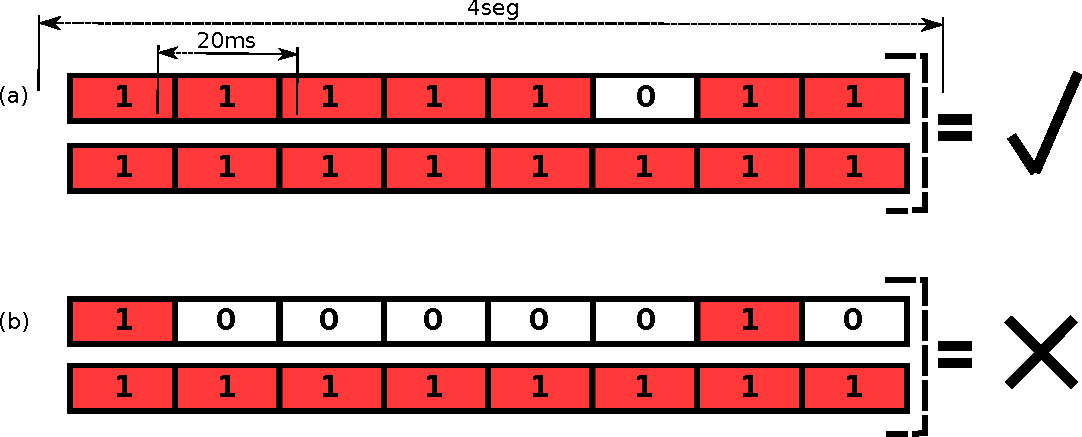
\includegraphics[width=0.8\textwidth]{integracion_temporal} 
\caption{Esquema de la integración temporal de las ventanas de analisis un fragmento de audio mayor, se ejemplifica con dos valores particulares en segundos. En rojo los audios detectados como no fondo, en blanco los que pertenencen al fondo según la etapa anterior. En (a) se observa un audio que pasa a la segunda etapa de clasificación, en (b) lo contrario.}
\label{fig:integracion_temporal}
\end{center}
\end{figure}
 
\subsubsection{Clasificación Sirena}

\subsubsection*{Extracción de Características}
Se utilizan al igual que en la publicacion \cite{Salamon:UrbanSound:ACMMM:14} los coeficientes MFCC (Mel-Frequency Cepstral Coeficients. 

For all the following experiments, we extracted Mel-Frequency Cepstral Coefficients (MFCC) from audio slices of \SI{20}{\milli\second} with 50\% frame overlap and hamming windowing. As in  work, we computed 40 Mel bands between 0 and \SI{22050}{\Hz} and kept the first 25 coefficients. 

\subsubsection*{Entrenamiento y Clasificación}


%----------------------------------------------------------------------------------------
%	SECTION 4
%----------------------------------------------------------------------------------------

\section{Conclusions}

The atomic weight of magnesium is concluded to be \SI{24}{\gram\per\mol}, as determined by the stoichiometry of its chemical combination with oxygen. This result is in agreement with the accepted value.


%----------------------------------------------------------------------------------------
%	BIBLIOGRAPHY
%----------------------------------------------------------------------------------------

\bibliographystyle{apalike}
\bibliography{sample}

%----------------------------------------------------------------------------------------
\end{document}